\documentclass[10pt,a4paper,notitlepage]{article}
\usepackage[latin1]{inputenc}
\usepackage{amsmath}
\usepackage{amsfonts}
\usepackage{amssymb}
\usepackage{graphicx}
\begin{document}

\title{jInfer Architecture} 
\author{Matej Vit�sek} 
\maketitle 

The description of jInfer architecture will commence by describing the data structures, namely representations of regular expressions and XML elements, attributes and simple data.\\

Afterwards the interfaces of basic inference modules - Initial Grammar Generator, Simplifier and Schema Generator - will be explained.\\

Finally, the process of inference will be described.

\subsection{Package naming conventions}

All packages start with \texttt{cz.cuni.mff.ksi.jinfer}. Afterwards is the short, normalized name of the module (e.g. \texttt{base}) and finally the package structure in this module (e.g. \texttt{objects.utils}). All in all, a package in the Base module could look like 
\begin{verbatim}
cz.cuni.mff.ksi.jinfer.base.objects.utils
\end{verbatim}

\section{Data structures}

\subsection{Regular expressions}

For general information on regular expressions, please refer for example to Wikipedia: $http://en.wikipedia.org/wiki/Regular\_expression$ .\\

All classes pertaining to regular expressions can be found in the package \texttt{cz.cuni.mff.ksi.jinfer.base.regexp}.\\

In jInfer, the following types of regular expressions are represented:
\begin{itemize}
	\item Token - a letter of the language described by this regular expression. In this case, an \texttt{AbstractNode} (see \ref{xml-rep}). Eg. \textit{"a"}.
	\item Concatenation - one or more regular expression in an ordered sequence. Eg. \textit{"(a, b, c, d)"}.
	\item Alternation - a choice between one or more regular expressions. Eg. \textit{"(a $|$ b $|$ c $|$ d)"}.
	\item Kleene star ("*") - a regular expression that can occur any number times (zero to infinity) in a row. Eg. \textit{"a*"}.
\end{itemize}

These types are defined in the \texttt{RegexpType} enum as \texttt{TOKEN}, \texttt{CONCATENATION}, \texttt{ALTERNATION} and \texttt{KLEENE}.\\

The class representing a regular expression is \texttt{Regexp}. A \texttt{Regexp} is a generic class (let's denominate its type variable as \textit{T}) that has three main members:
\begin{itemize}
	\item \texttt{type} - a \texttt{RegexpType} instance, set in the constructor and immutable afterwards. Can be queried via the method \texttt{getType()} or shorthand boolean methods
	\begin{itemize}
		\item \texttt{isToken()}
		\item \texttt{isConcatenation()}
		\item \texttt{isAlternation()}
		\item \texttt{isKleene()}
	\end{itemize}
	
	\item \texttt{content} - a type \textit{T} member. Must be set iff the \texttt{type} is \texttt{TOKEN}, \texttt{null} otherwise. Means "the token represented by this regular expression". % TODO how to query
	
	\item \texttt{children} - a list of \texttt{Regexp}s of the type \textit{T}. Must be set iff the \texttt{type} is \textbf{not} \texttt{TOKEN}, \texttt{null} otherwise. If the \texttt{type} is \texttt{KLEENE}, it must contain exactly one element, although this rule is not enforced by the code. Otherwise the number of elements in this list is unconstrained. The meaning of this member is "the list of regular sub-expressions in this concatenation / alternation / Kleene star". % TODO how to query
\end{itemize}

\textit{Example:} regular expression \textit{"(a, b, (c $|$ d))*"} would be represented as a \texttt{Regexp} of type \texttt{KLEENE} with children of size 1, containing a \texttt{CONCATENATION} with 3 children. Of these three, the first two would be \texttt{TOKEN}s with content \textit{"a"} and \textit{"b"} respectively. The last child would be an \texttt{ALTERNATION} containing two \texttt{TOKEN}s \textit{"c"} and \textit{"d"}. It is obvious that this representation of regular expressions creates tree structures.

\subsection{XML representation}
\label{xml-rep}

The classes that represent XML elements, attributes and simple text data are summarized in figure \ref{img-arch-nodes}.

\begin{figure}
	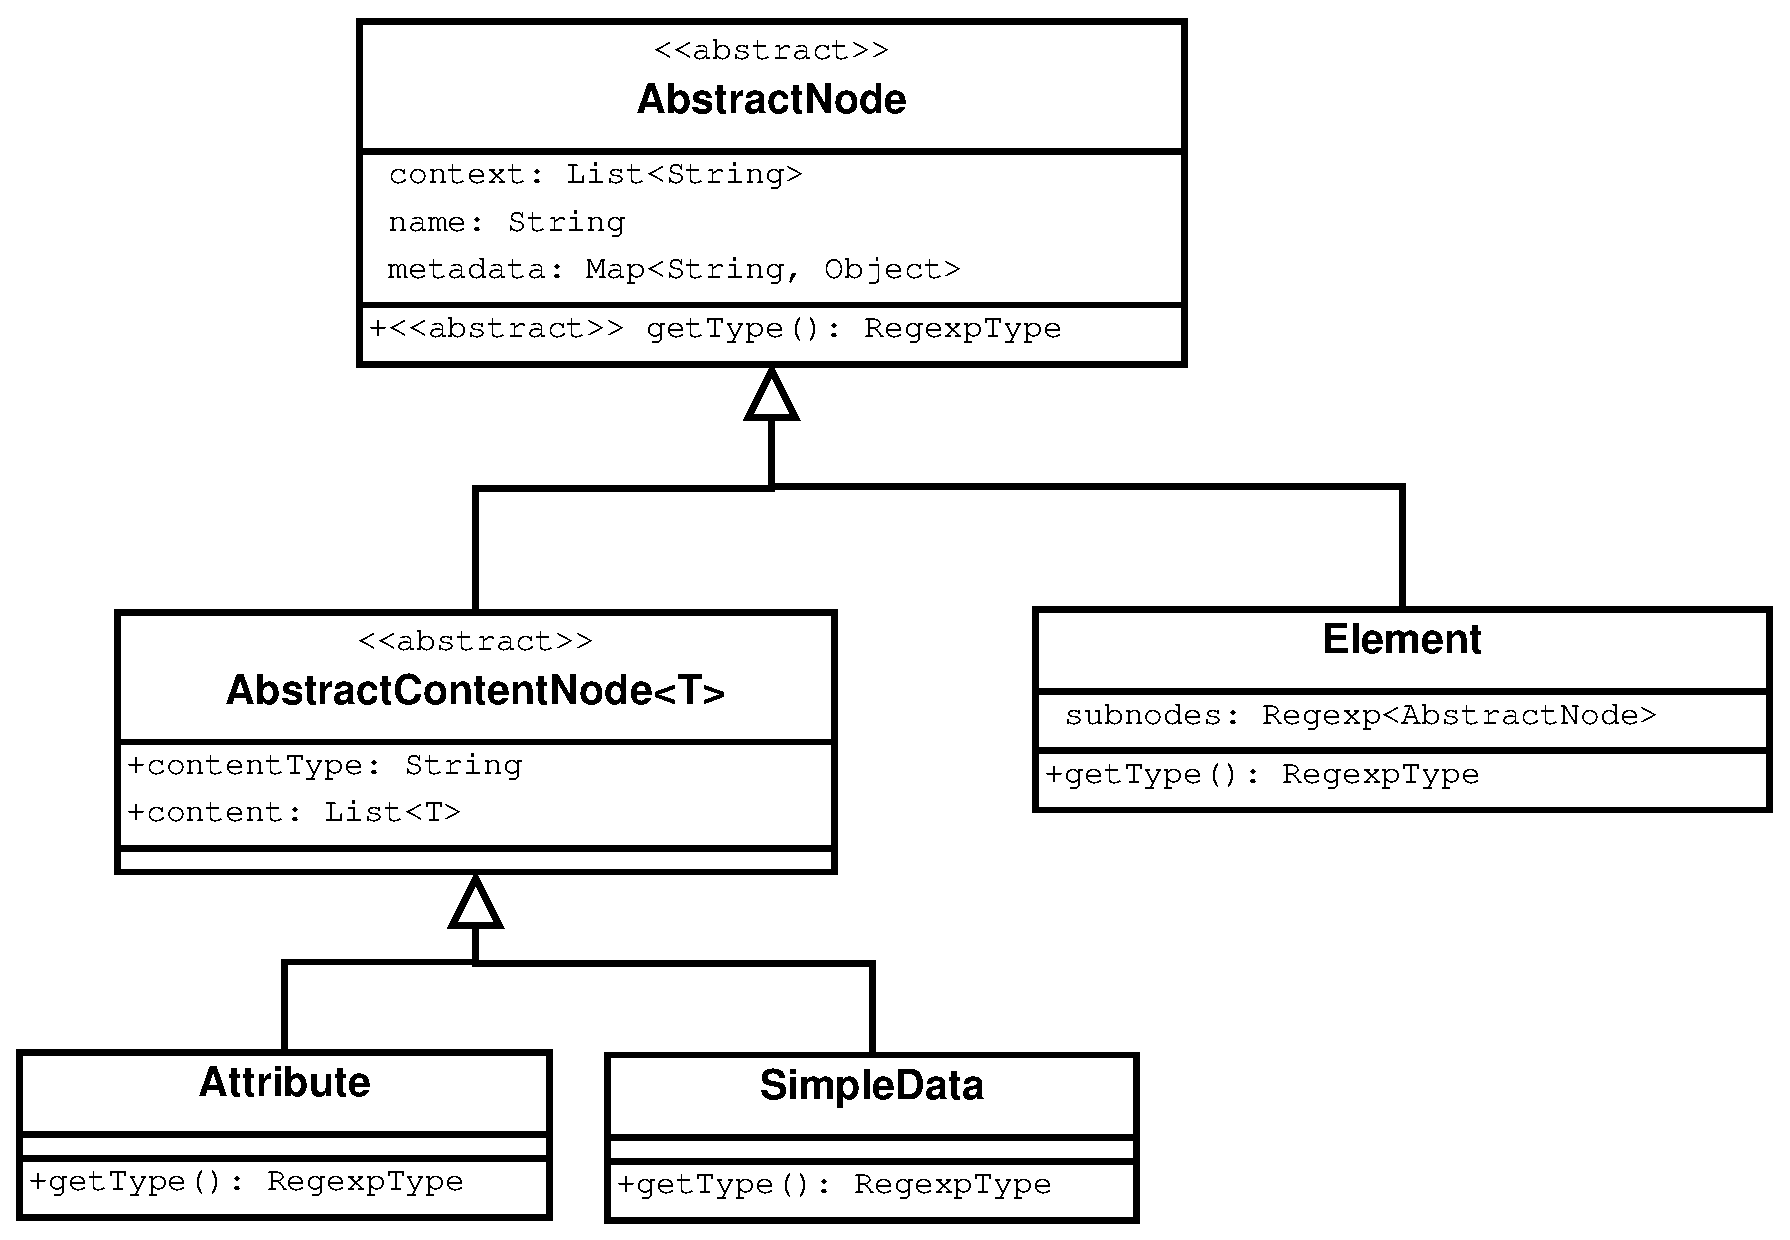
\includegraphics[scale=0.3]{Architecture-images/nodes.eps} 
	\caption{UML class diagram of classes representing parts of XML}
	\label{img-arch-nodes}
\end{figure}

It is important to note that attributes in jInfer's data structures are nodes, just like elements and simple data.\\

Description of all classes from the schema follows.

\subsubsection{AbstractNode}

\subsubsection{Element}

\subsubsection{AbstractContentNode}

\subsubsection{Attribute}

\subsubsection{SimpleData}

\section{Interfaces}

\section{Inference process}

\end{document}